\documentclass[twoside]{book}

% Packages required by doxygen
\usepackage{fixltx2e}
\usepackage{calc}
\usepackage{doxygen}
\usepackage[export]{adjustbox} % also loads graphicx
\usepackage{graphicx}
\usepackage[utf8]{inputenc}
\usepackage{makeidx}
\usepackage{multicol}
\usepackage{multirow}
\PassOptionsToPackage{warn}{textcomp}
\usepackage{textcomp}
\usepackage[nointegrals]{wasysym}
\usepackage[table]{xcolor}

% Font selection
\usepackage[T1]{fontenc}
\usepackage[scaled=.90]{helvet}
\usepackage{courier}
\usepackage{amssymb}
\usepackage{sectsty}
\renewcommand{\familydefault}{\sfdefault}
\allsectionsfont{%
  \fontseries{bc}\selectfont%
  \color{darkgray}%
}
\renewcommand{\DoxyLabelFont}{%
  \fontseries{bc}\selectfont%
  \color{darkgray}%
}
\newcommand{\+}{\discretionary{\mbox{\scriptsize$\hookleftarrow$}}{}{}}

% Page & text layout
\usepackage{geometry}
\geometry{%
  a4paper,%
  top=2.5cm,%
  bottom=2.5cm,%
  left=2.5cm,%
  right=2.5cm%
}
\tolerance=750
\hfuzz=15pt
\hbadness=750
\setlength{\emergencystretch}{15pt}
\setlength{\parindent}{0cm}
\setlength{\parskip}{3ex plus 2ex minus 2ex}
\makeatletter
\renewcommand{\paragraph}{%
  \@startsection{paragraph}{4}{0ex}{-1.0ex}{1.0ex}{%
    \normalfont\normalsize\bfseries\SS@parafont%
  }%
}
\renewcommand{\subparagraph}{%
  \@startsection{subparagraph}{5}{0ex}{-1.0ex}{1.0ex}{%
    \normalfont\normalsize\bfseries\SS@subparafont%
  }%
}
\makeatother

% Headers & footers
\usepackage{fancyhdr}
\pagestyle{fancyplain}
\fancyhead[LE]{\fancyplain{}{\bfseries\thepage}}
\fancyhead[CE]{\fancyplain{}{}}
\fancyhead[RE]{\fancyplain{}{\bfseries\leftmark}}
\fancyhead[LO]{\fancyplain{}{\bfseries\rightmark}}
\fancyhead[CO]{\fancyplain{}{}}
\fancyhead[RO]{\fancyplain{}{\bfseries\thepage}}
\fancyfoot[LE]{\fancyplain{}{}}
\fancyfoot[CE]{\fancyplain{}{}}
\fancyfoot[RE]{\fancyplain{}{\bfseries\scriptsize Generated by Doxygen }}
\fancyfoot[LO]{\fancyplain{}{\bfseries\scriptsize Generated by Doxygen }}
\fancyfoot[CO]{\fancyplain{}{}}
\fancyfoot[RO]{\fancyplain{}{}}
\renewcommand{\footrulewidth}{0.4pt}
\renewcommand{\chaptermark}[1]{%
  \markboth{#1}{}%
}
\renewcommand{\sectionmark}[1]{%
  \markright{\thesection\ #1}%
}

% Indices & bibliography
\usepackage{natbib}
\usepackage[titles]{tocloft}
\setcounter{tocdepth}{3}
\setcounter{secnumdepth}{5}
\makeindex

% Hyperlinks (required, but should be loaded last)
\usepackage{ifpdf}
\ifpdf
  \usepackage[pdftex,pagebackref=true]{hyperref}
\else
  \usepackage[ps2pdf,pagebackref=true]{hyperref}
\fi
\hypersetup{%
  colorlinks=true,%
  linkcolor=blue,%
  citecolor=blue,%
  unicode%
}

% Custom commands
\newcommand{\clearemptydoublepage}{%
  \newpage{\pagestyle{empty}\cleardoublepage}%
}

\usepackage{caption}
\captionsetup{labelsep=space,justification=centering,font={bf},singlelinecheck=off,skip=4pt,position=top}

%===== C O N T E N T S =====

\begin{document}

% Titlepage & ToC
\hypersetup{pageanchor=false,
             bookmarksnumbered=true,
             pdfencoding=unicode
            }
\pagenumbering{roman}
\begin{titlepage}
\vspace*{7cm}
\begin{center}%
{\Large My Project }\\
\vspace*{1cm}
{\large Generated by Doxygen 1.8.11}\\
\end{center}
\end{titlepage}
\clearemptydoublepage
\tableofcontents
\clearemptydoublepage
\pagenumbering{arabic}
\hypersetup{pageanchor=true}

%--- Begin generated contents ---
\chapter{File Index}
\section{File List}
Here is a list of all files with brief descriptions\+:\begin{DoxyCompactList}
\item\contentsline{section}{\hyperlink{Lab1_8c}{Lab1.\+c} }{\pageref{Lab1_8c}}{}
\end{DoxyCompactList}

\chapter{File Documentation}
\hypertarget{SegmentedSieve_8cpp}{}\section{Segmented\+Sieve.\+cpp File Reference}
\label{SegmentedSieve_8cpp}\index{Segmented\+Sieve.\+cpp@{Segmented\+Sieve.\+cpp}}
{\ttfamily \#include $<$iostream$>$}\\*
{\ttfamily \#include $<$cstring$>$}\\*
Include dependency graph for Segmented\+Sieve.\+cpp\+:
\nopagebreak
\begin{figure}[H]
\begin{center}
\leavevmode
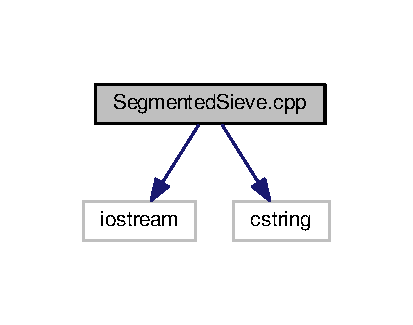
\includegraphics[width=198pt]{SegmentedSieve_8cpp__incl}
\end{center}
\end{figure}
\subsection*{Macros}
\begin{DoxyCompactItemize}
\item 
\#define \hyperlink{SegmentedSieve_8cpp_a392fb874e547e582e9c66a08a1f23326}{M\+AX}~46656
\item 
\#define \hyperlink{SegmentedSieve_8cpp_a9380b96a9d86a7a13b0a77251cd78a08}{L\+MT}~216
\item 
\#define \hyperlink{SegmentedSieve_8cpp_a05b49c662c073f89e86804f7856622a0}{L\+EN}~4830
\item 
\#define \hyperlink{SegmentedSieve_8cpp_a5b0885b8b55bbc13691092b704d9309f}{R\+NG}~100032
\item 
\#define \hyperlink{SegmentedSieve_8cpp_ae7616788b30810a219d9cdee95904ba4}{sq}(x)~((x)$\ast$(x))
\item 
\#define \hyperlink{SegmentedSieve_8cpp_a35340c244a894d128c016ea0c36ba7cd}{mset}(x,  v)~memset(x, v , sizeof(x))
\item 
\#define \hyperlink{SegmentedSieve_8cpp_aef23bd3f4e80c89a8ac8bba2bca913f6}{chkC}(x,  n)~(x\mbox{[}n $>$$>$ 6\mbox{]} \& (1 $<$$<$ ((n $>$$>$ 1) \& 31)))
\item 
\#define \hyperlink{SegmentedSieve_8cpp_a7131ce61f65d045c53abbfa0627a64b3}{setC}(x,  n)~(x\mbox{[}n $>$$>$ 6\mbox{]} $\vert$= (1 $<$$<$ ((n $>$$>$ 1) \& 31)))
\end{DoxyCompactItemize}
\subsection*{Functions}
\begin{DoxyCompactItemize}
\item 
void \hyperlink{SegmentedSieve_8cpp_a111c45486d29e23ca8d5a8a2e1c6436e}{sieve} ()
\item 
int \hyperlink{SegmentedSieve_8cpp_a4d3f608185b771d2499c1c9494f2fe16}{segmented\+\_\+sieve} (int a, int b)
\item 
int \hyperlink{SegmentedSieve_8cpp_ae66f6b31b5ad750f1fe042a706a4e3d4}{main} ()
\end{DoxyCompactItemize}
\subsection*{Variables}
\begin{DoxyCompactItemize}
\item 
unsigned \hyperlink{SegmentedSieve_8cpp_a4ba4f1c54d9400b3a1c3be1a3cf8352f}{base} \mbox{[}\hyperlink{SegmentedSieve_8cpp_a392fb874e547e582e9c66a08a1f23326}{M\+AX}/64\mbox{]}
\item 
unsigned \hyperlink{SegmentedSieve_8cpp_a8bed8ce91ccb458d3373b913afd8712e}{segment} \mbox{[}\hyperlink{SegmentedSieve_8cpp_a5b0885b8b55bbc13691092b704d9309f}{R\+NG}/64\mbox{]}
\item 
unsigned \hyperlink{SegmentedSieve_8cpp_aa3306f7e7367c34600079c5542f67c37}{primes} \mbox{[}\hyperlink{SegmentedSieve_8cpp_a05b49c662c073f89e86804f7856622a0}{L\+EN}\mbox{]}
\end{DoxyCompactItemize}


\subsection{Macro Definition Documentation}
\index{Segmented\+Sieve.\+cpp@{Segmented\+Sieve.\+cpp}!chkC@{chkC}}
\index{chkC@{chkC}!Segmented\+Sieve.\+cpp@{Segmented\+Sieve.\+cpp}}
\subsubsection[{\texorpdfstring{chkC}{chkC}}]{\setlength{\rightskip}{0pt plus 5cm}\#define chkC(
\begin{DoxyParamCaption}
\item[{}]{x, }
\item[{}]{n}
\end{DoxyParamCaption}
)~(x\mbox{[}n $>$$>$ 6\mbox{]} \& (1 $<$$<$ ((n $>$$>$ 1) \& 31)))}\hypertarget{SegmentedSieve_8cpp_aef23bd3f4e80c89a8ac8bba2bca913f6}{}\label{SegmentedSieve_8cpp_aef23bd3f4e80c89a8ac8bba2bca913f6}
\index{Segmented\+Sieve.\+cpp@{Segmented\+Sieve.\+cpp}!L\+EN@{L\+EN}}
\index{L\+EN@{L\+EN}!Segmented\+Sieve.\+cpp@{Segmented\+Sieve.\+cpp}}
\subsubsection[{\texorpdfstring{L\+EN}{LEN}}]{\setlength{\rightskip}{0pt plus 5cm}\#define L\+EN~4830}\hypertarget{SegmentedSieve_8cpp_a05b49c662c073f89e86804f7856622a0}{}\label{SegmentedSieve_8cpp_a05b49c662c073f89e86804f7856622a0}
\index{Segmented\+Sieve.\+cpp@{Segmented\+Sieve.\+cpp}!L\+MT@{L\+MT}}
\index{L\+MT@{L\+MT}!Segmented\+Sieve.\+cpp@{Segmented\+Sieve.\+cpp}}
\subsubsection[{\texorpdfstring{L\+MT}{LMT}}]{\setlength{\rightskip}{0pt plus 5cm}\#define L\+MT~216}\hypertarget{SegmentedSieve_8cpp_a9380b96a9d86a7a13b0a77251cd78a08}{}\label{SegmentedSieve_8cpp_a9380b96a9d86a7a13b0a77251cd78a08}
\index{Segmented\+Sieve.\+cpp@{Segmented\+Sieve.\+cpp}!M\+AX@{M\+AX}}
\index{M\+AX@{M\+AX}!Segmented\+Sieve.\+cpp@{Segmented\+Sieve.\+cpp}}
\subsubsection[{\texorpdfstring{M\+AX}{MAX}}]{\setlength{\rightskip}{0pt plus 5cm}\#define M\+AX~46656}\hypertarget{SegmentedSieve_8cpp_a392fb874e547e582e9c66a08a1f23326}{}\label{SegmentedSieve_8cpp_a392fb874e547e582e9c66a08a1f23326}
\index{Segmented\+Sieve.\+cpp@{Segmented\+Sieve.\+cpp}!mset@{mset}}
\index{mset@{mset}!Segmented\+Sieve.\+cpp@{Segmented\+Sieve.\+cpp}}
\subsubsection[{\texorpdfstring{mset}{mset}}]{\setlength{\rightskip}{0pt plus 5cm}\#define mset(
\begin{DoxyParamCaption}
\item[{}]{x, }
\item[{}]{v}
\end{DoxyParamCaption}
)~memset(x, v , sizeof(x))}\hypertarget{SegmentedSieve_8cpp_a35340c244a894d128c016ea0c36ba7cd}{}\label{SegmentedSieve_8cpp_a35340c244a894d128c016ea0c36ba7cd}
\index{Segmented\+Sieve.\+cpp@{Segmented\+Sieve.\+cpp}!R\+NG@{R\+NG}}
\index{R\+NG@{R\+NG}!Segmented\+Sieve.\+cpp@{Segmented\+Sieve.\+cpp}}
\subsubsection[{\texorpdfstring{R\+NG}{RNG}}]{\setlength{\rightskip}{0pt plus 5cm}\#define R\+NG~100032}\hypertarget{SegmentedSieve_8cpp_a5b0885b8b55bbc13691092b704d9309f}{}\label{SegmentedSieve_8cpp_a5b0885b8b55bbc13691092b704d9309f}
\index{Segmented\+Sieve.\+cpp@{Segmented\+Sieve.\+cpp}!setC@{setC}}
\index{setC@{setC}!Segmented\+Sieve.\+cpp@{Segmented\+Sieve.\+cpp}}
\subsubsection[{\texorpdfstring{setC}{setC}}]{\setlength{\rightskip}{0pt plus 5cm}\#define setC(
\begin{DoxyParamCaption}
\item[{}]{x, }
\item[{}]{n}
\end{DoxyParamCaption}
)~(x\mbox{[}n $>$$>$ 6\mbox{]} $\vert$= (1 $<$$<$ ((n $>$$>$ 1) \& 31)))}\hypertarget{SegmentedSieve_8cpp_a7131ce61f65d045c53abbfa0627a64b3}{}\label{SegmentedSieve_8cpp_a7131ce61f65d045c53abbfa0627a64b3}
\index{Segmented\+Sieve.\+cpp@{Segmented\+Sieve.\+cpp}!sq@{sq}}
\index{sq@{sq}!Segmented\+Sieve.\+cpp@{Segmented\+Sieve.\+cpp}}
\subsubsection[{\texorpdfstring{sq}{sq}}]{\setlength{\rightskip}{0pt plus 5cm}\#define sq(
\begin{DoxyParamCaption}
\item[{}]{x}
\end{DoxyParamCaption}
)~((x)$\ast$(x))}\hypertarget{SegmentedSieve_8cpp_ae7616788b30810a219d9cdee95904ba4}{}\label{SegmentedSieve_8cpp_ae7616788b30810a219d9cdee95904ba4}


\subsection{Function Documentation}
\index{Segmented\+Sieve.\+cpp@{Segmented\+Sieve.\+cpp}!main@{main}}
\index{main@{main}!Segmented\+Sieve.\+cpp@{Segmented\+Sieve.\+cpp}}
\subsubsection[{\texorpdfstring{main()}{main()}}]{\setlength{\rightskip}{0pt plus 5cm}int main (
\begin{DoxyParamCaption}
{}
\end{DoxyParamCaption}
)}\hypertarget{SegmentedSieve_8cpp_ae66f6b31b5ad750f1fe042a706a4e3d4}{}\label{SegmentedSieve_8cpp_ae66f6b31b5ad750f1fe042a706a4e3d4}

\begin{DoxyCode}
72 \{
73     \hyperlink{SegmentedSieve_8cpp_a111c45486d29e23ca8d5a8a2e1c6436e}{sieve}();
74     \textcolor{keywordtype}{int} a, b;
75     cout<<\textcolor{stringliteral}{"Enter Lower Bound: "};
76     cin>>a;
77     cout<<\textcolor{stringliteral}{"Enter Upper Bound: "};
78     cin>>b;
79     cout<<\textcolor{stringliteral}{"Number of primes between "}<<a<<\textcolor{stringliteral}{" and "}<<b<<\textcolor{stringliteral}{":  "};
80     cout<<\hyperlink{SegmentedSieve_8cpp_a4d3f608185b771d2499c1c9494f2fe16}{segmented\_sieve}(a, b)<<endl;
81     \textcolor{keywordflow}{return} 0;
82 \}
\end{DoxyCode}


Here is the call graph for this function\+:
\nopagebreak
\begin{figure}[H]
\begin{center}
\leavevmode
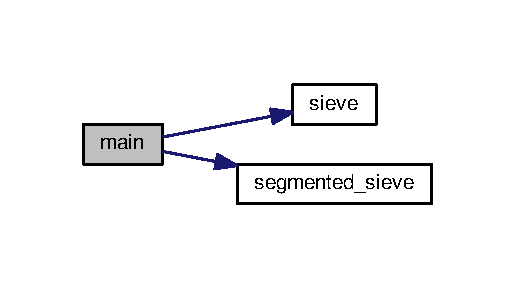
\includegraphics[width=247pt]{SegmentedSieve_8cpp_ae66f6b31b5ad750f1fe042a706a4e3d4_cgraph}
\end{center}
\end{figure}


\index{Segmented\+Sieve.\+cpp@{Segmented\+Sieve.\+cpp}!segmented\+\_\+sieve@{segmented\+\_\+sieve}}
\index{segmented\+\_\+sieve@{segmented\+\_\+sieve}!Segmented\+Sieve.\+cpp@{Segmented\+Sieve.\+cpp}}
\subsubsection[{\texorpdfstring{segmented\+\_\+sieve(int a, int b)}{segmented_sieve(int a, int b)}}]{\setlength{\rightskip}{0pt plus 5cm}int segmented\+\_\+sieve (
\begin{DoxyParamCaption}
\item[{int}]{a, }
\item[{int}]{b}
\end{DoxyParamCaption}
)}\hypertarget{SegmentedSieve_8cpp_a4d3f608185b771d2499c1c9494f2fe16}{}\label{SegmentedSieve_8cpp_a4d3f608185b771d2499c1c9494f2fe16}

\begin{DoxyCode}
42 \{
43     \textcolor{keywordtype}{unsigned} i, j, k, cnt = (a <= 2 && 2 <=b )? 1 : 0;
44     \textcolor{keywordflow}{if} (b < 2) 
45         \textcolor{keywordflow}{return} 0;
46     \textcolor{keywordflow}{if} (a < 3) 
47         a = 3;
48     \textcolor{keywordflow}{if} (a % 2 == 0) 
49         a++;
50     \hyperlink{SegmentedSieve_8cpp_a35340c244a894d128c016ea0c36ba7cd}{mset} (\hyperlink{SegmentedSieve_8cpp_a8bed8ce91ccb458d3373b913afd8712e}{segment}, 0);
51     \textcolor{keywordflow}{for} (i = 0; \hyperlink{SegmentedSieve_8cpp_ae7616788b30810a219d9cdee95904ba4}{sq}(\hyperlink{SegmentedSieve_8cpp_aa3306f7e7367c34600079c5542f67c37}{primes}[i]) <= b; i++)
52     \{
53         j = \hyperlink{SegmentedSieve_8cpp_aa3306f7e7367c34600079c5542f67c37}{primes}[i] * ((a + \hyperlink{SegmentedSieve_8cpp_aa3306f7e7367c34600079c5542f67c37}{primes}[i] - 1) / \hyperlink{SegmentedSieve_8cpp_aa3306f7e7367c34600079c5542f67c37}{primes}[i]);
54         \textcolor{keywordflow}{if} (j % 2 == 0) j += \hyperlink{SegmentedSieve_8cpp_aa3306f7e7367c34600079c5542f67c37}{primes}[i];
55         \textcolor{keywordflow}{for} (k = \hyperlink{SegmentedSieve_8cpp_aa3306f7e7367c34600079c5542f67c37}{primes}[i] << 1; j <= b; j += k)
56         \{
57             \textcolor{keywordflow}{if} (j != \hyperlink{SegmentedSieve_8cpp_aa3306f7e7367c34600079c5542f67c37}{primes}[i])
58                 \hyperlink{SegmentedSieve_8cpp_a7131ce61f65d045c53abbfa0627a64b3}{setC}(\hyperlink{SegmentedSieve_8cpp_a8bed8ce91ccb458d3373b913afd8712e}{segment}, (j - a));
59         \}
60     \}
61     \textcolor{keywordflow}{for} (i = 0; i <= b - a; i += 2)
62     \{
63         \textcolor{keywordflow}{if} (!\hyperlink{SegmentedSieve_8cpp_aef23bd3f4e80c89a8ac8bba2bca913f6}{chkC}(\hyperlink{SegmentedSieve_8cpp_a8bed8ce91ccb458d3373b913afd8712e}{segment}, i))
64             cnt++;
65     \}
66     \textcolor{keywordflow}{return} cnt;
67 \}
\end{DoxyCode}
\index{Segmented\+Sieve.\+cpp@{Segmented\+Sieve.\+cpp}!sieve@{sieve}}
\index{sieve@{sieve}!Segmented\+Sieve.\+cpp@{Segmented\+Sieve.\+cpp}}
\subsubsection[{\texorpdfstring{sieve()}{sieve()}}]{\setlength{\rightskip}{0pt plus 5cm}void sieve (
\begin{DoxyParamCaption}
{}
\end{DoxyParamCaption}
)}\hypertarget{SegmentedSieve_8cpp_a111c45486d29e23ca8d5a8a2e1c6436e}{}\label{SegmentedSieve_8cpp_a111c45486d29e23ca8d5a8a2e1c6436e}

\begin{DoxyCode}
21 \{
22     \textcolor{keywordtype}{unsigned} i, j, k;
23     \textcolor{keywordflow}{for} (i = 3; i < \hyperlink{SegmentedSieve_8cpp_a9380b96a9d86a7a13b0a77251cd78a08}{LMT}; i += 2)
24     \{
25         \textcolor{keywordflow}{if} (!\hyperlink{SegmentedSieve_8cpp_aef23bd3f4e80c89a8ac8bba2bca913f6}{chkC}(\hyperlink{SegmentedSieve_8cpp_a4ba4f1c54d9400b3a1c3be1a3cf8352f}{base}, i))
26         \{    
27             \textcolor{keywordflow}{for} (j = i * i, k = i << 1; j < \hyperlink{SegmentedSieve_8cpp_a392fb874e547e582e9c66a08a1f23326}{MAX}; j += k)
28                 \hyperlink{SegmentedSieve_8cpp_a7131ce61f65d045c53abbfa0627a64b3}{setC}(\hyperlink{SegmentedSieve_8cpp_a4ba4f1c54d9400b3a1c3be1a3cf8352f}{base}, j);
29         \}
30     \}
31     \textcolor{keywordflow}{for} (i = 3, j = 0; i < \hyperlink{SegmentedSieve_8cpp_a392fb874e547e582e9c66a08a1f23326}{MAX}; i += 2)
32     \{
33         \textcolor{keywordflow}{if} (!\hyperlink{SegmentedSieve_8cpp_aef23bd3f4e80c89a8ac8bba2bca913f6}{chkC}(\hyperlink{SegmentedSieve_8cpp_a4ba4f1c54d9400b3a1c3be1a3cf8352f}{base}, i))
34             \hyperlink{SegmentedSieve_8cpp_aa3306f7e7367c34600079c5542f67c37}{primes}[j++] = i;
35     \}
36 \}
\end{DoxyCode}


\subsection{Variable Documentation}
\index{Segmented\+Sieve.\+cpp@{Segmented\+Sieve.\+cpp}!base@{base}}
\index{base@{base}!Segmented\+Sieve.\+cpp@{Segmented\+Sieve.\+cpp}}
\subsubsection[{\texorpdfstring{base}{base}}]{\setlength{\rightskip}{0pt plus 5cm}unsigned base\mbox{[}{\bf M\+AX}/64\mbox{]}}\hypertarget{SegmentedSieve_8cpp_a4ba4f1c54d9400b3a1c3be1a3cf8352f}{}\label{SegmentedSieve_8cpp_a4ba4f1c54d9400b3a1c3be1a3cf8352f}
\index{Segmented\+Sieve.\+cpp@{Segmented\+Sieve.\+cpp}!primes@{primes}}
\index{primes@{primes}!Segmented\+Sieve.\+cpp@{Segmented\+Sieve.\+cpp}}
\subsubsection[{\texorpdfstring{primes}{primes}}]{\setlength{\rightskip}{0pt plus 5cm}unsigned primes\mbox{[}{\bf L\+EN}\mbox{]}}\hypertarget{SegmentedSieve_8cpp_aa3306f7e7367c34600079c5542f67c37}{}\label{SegmentedSieve_8cpp_aa3306f7e7367c34600079c5542f67c37}
\index{Segmented\+Sieve.\+cpp@{Segmented\+Sieve.\+cpp}!segment@{segment}}
\index{segment@{segment}!Segmented\+Sieve.\+cpp@{Segmented\+Sieve.\+cpp}}
\subsubsection[{\texorpdfstring{segment}{segment}}]{\setlength{\rightskip}{0pt plus 5cm}unsigned segment\mbox{[}{\bf R\+NG}/64\mbox{]}}\hypertarget{SegmentedSieve_8cpp_a8bed8ce91ccb458d3373b913afd8712e}{}\label{SegmentedSieve_8cpp_a8bed8ce91ccb458d3373b913afd8712e}

%--- End generated contents ---

% Index
\backmatter
\newpage
\phantomsection
\clearemptydoublepage
\addcontentsline{toc}{chapter}{Index}
\printindex

\end{document}
